\section{Sprints}
\begin{description}
	\item [Sprint 1] \hfill \\
	Im ersten Sprint sicherten wir die Grundfnktionalität. Im ersten Sprint wollten wir sicher gehen, dass die Verbindung zwischen Sensor, Basisstation und App gewährleistet ist. Hierzu hatten wir folgende Kernpunkte:
	\begin{itemize}		
		\item App GUI Konzept 
		\item App GUI fertigstellen
		\item Verbindung zwischen Basisstation und App
		\item Verbindung zwischen Smart Gadget und Basisstation
		\item App GUI Grundgerüst
		\item Verbindung zwischen Smart Gadget und App verstehen
		\item Software-Layout Basisstation
		\item Benachrichtigung Push
		\item Klassen definieren die auf app und Basistation benutzt werden
		\item App Software Architektur Konzept
		\item Benachrichtigung
		\item Erstes Datenbankschema definieren
		\item Schnittstelle zwischen App und Basistation definieren
	\end{itemize}
	Wir konnten die Aufgaben wie in der Burndownchart ersichtlich fertigstellen.
	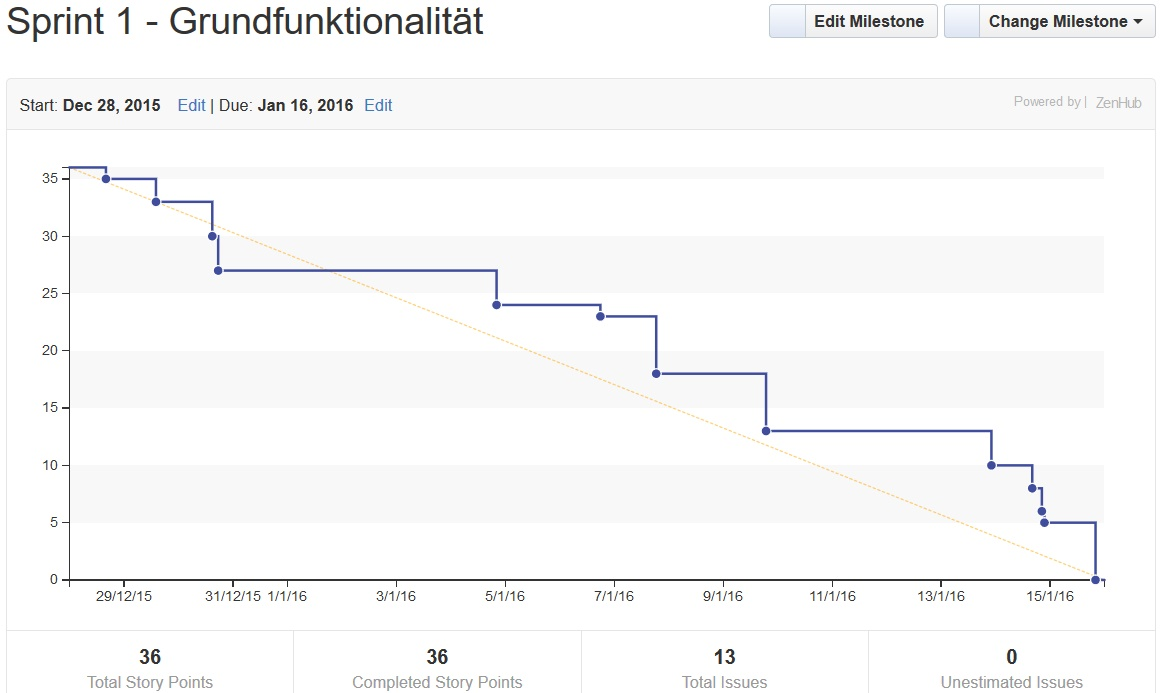
\includegraphics[width=0.7\textwidth]{burndown_sprint1.jpg}
	Innerhalb der App wurde die GUI fertig gestellt und sieht folgendermaßen aus:
	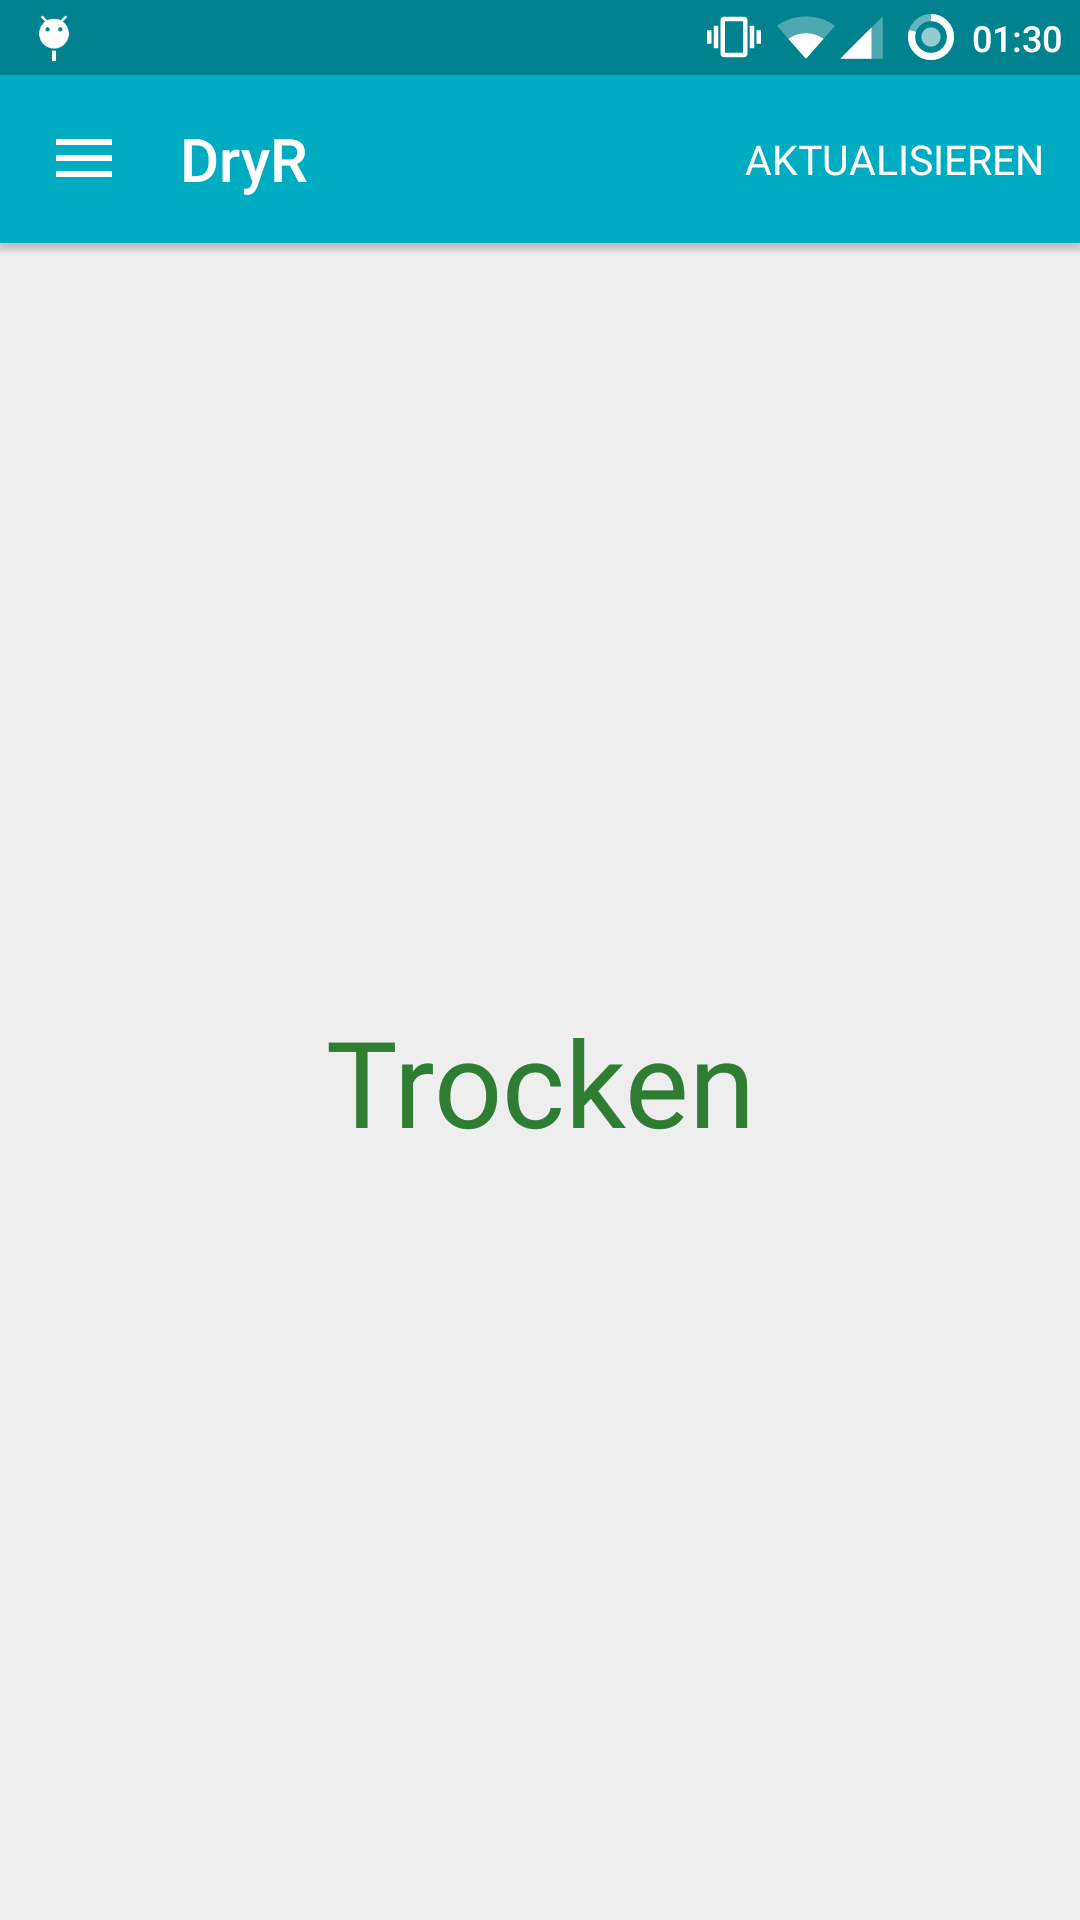
\includegraphics[width=0.7\textwidth]{laundry_status_dry.png}
	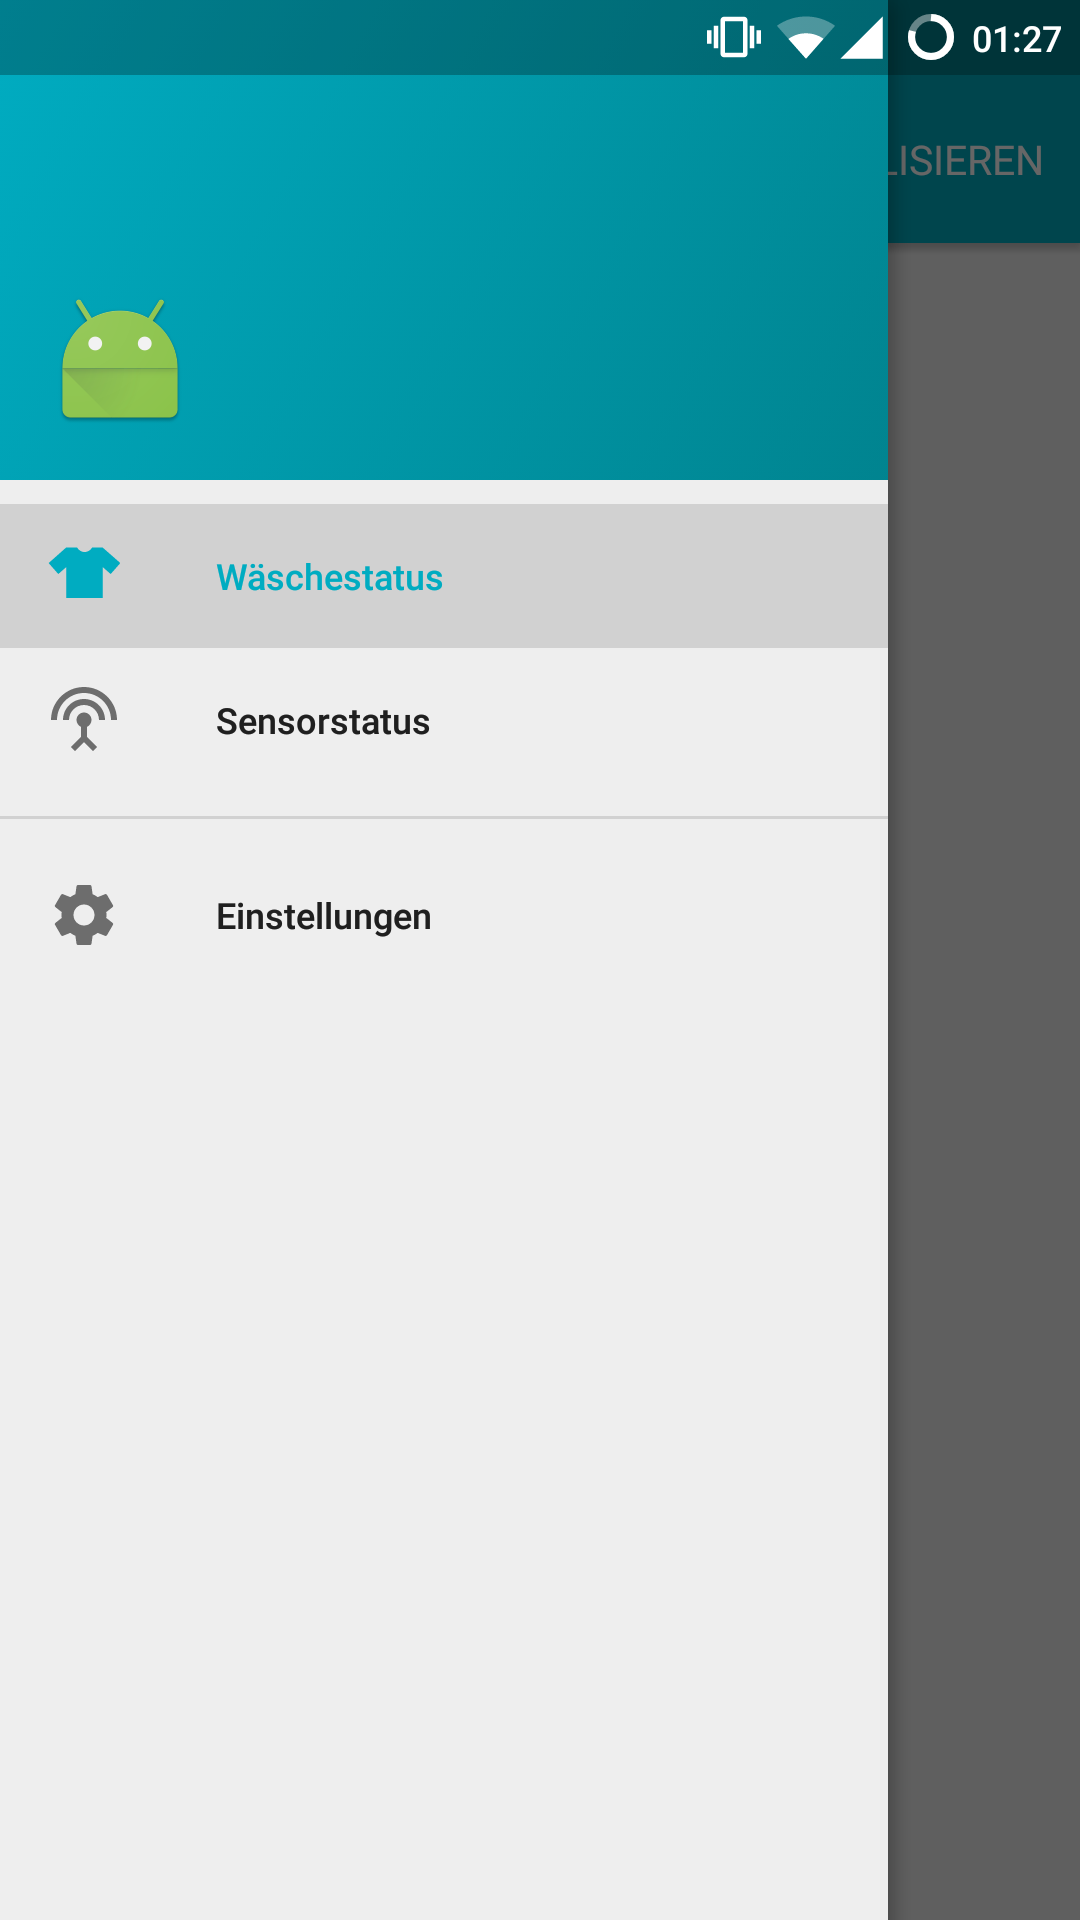
\includegraphics[width=0.7\textwidth]{nav_drawer.png}

	\item [Sprint 2] \hfill \\
		Im zweiten Sprint wollten wir die Benutzerfreundlichkeit erhöhen.
		Hierbei hat sich schnell heraus gestellt, dass einige Funktionalitäten mit der Hardware des Sensors nicht realisierbar sind. Die Platine lässt in ihrer jetzigen Bauart nicht zu, dass man den Ladezustand der Baterie mesen kann. Die Kernpunkte "Wäsche Trocken" und "Vorherage" haben wir somit bereits im 2. Sprint begonnen. Ein großes Thema war der Betrieb mehrer Sensoren 
		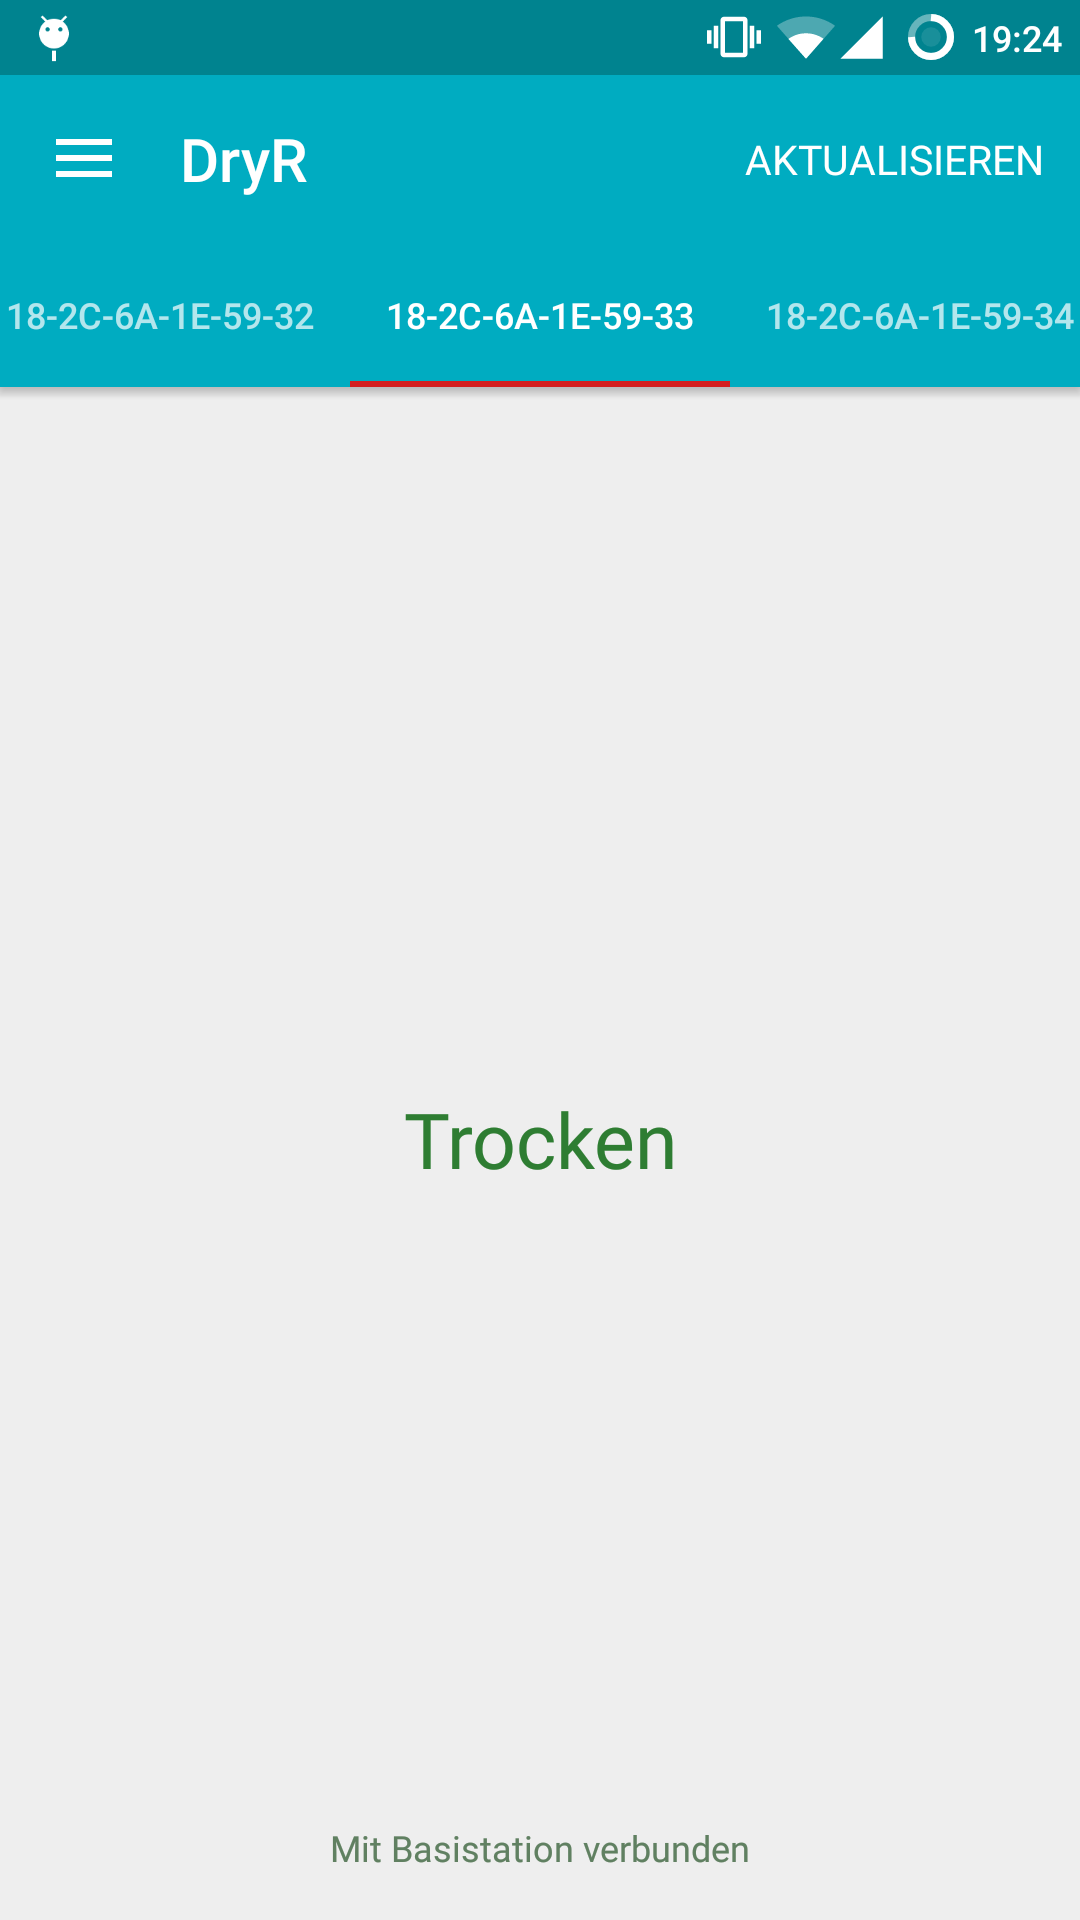
\includegraphics[width=0.7\textwidth]{laundry_status_multiple_sensors.png}
		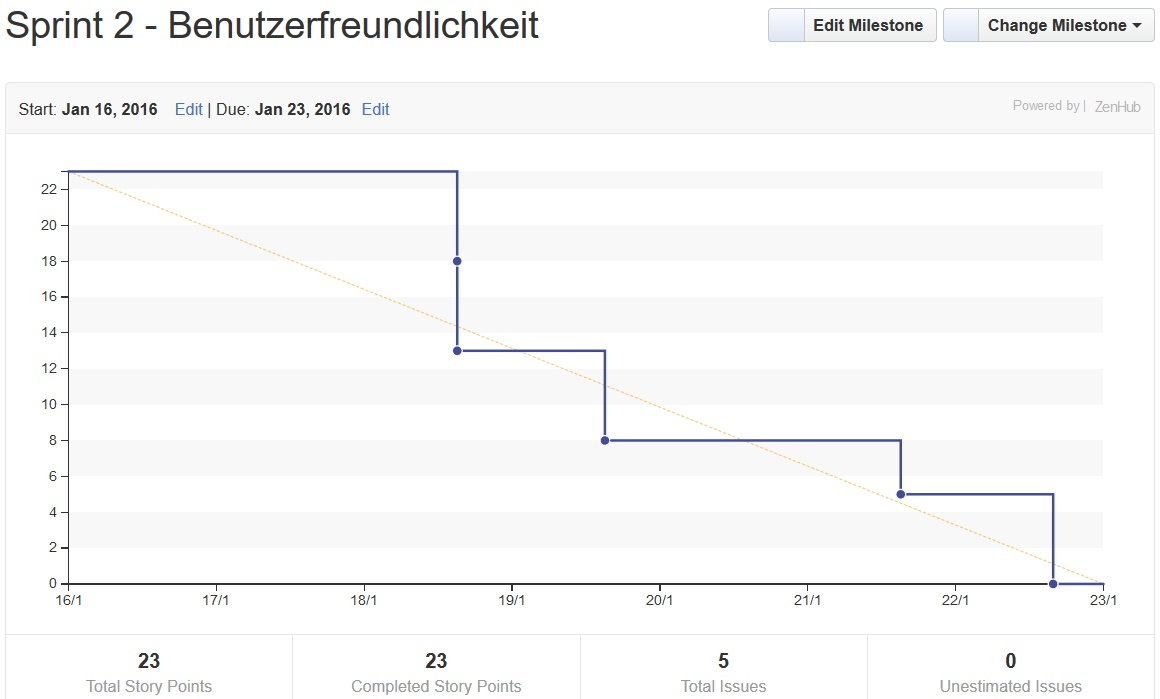
\includegraphics[width=0.7\textwidth]{burndown_sprint2.jpg}
	\item [Sprint 3] \hfill \\
		der 3. Sprint war wür weitere Features gedacht. 
		Jedoch hatten wir durch den Emulator und durch den Betrieb mehrer Sensorgeräte einige Probleme wodurch wir einige Features nicht realisiert haben und uns lieber auf Bugsuche begeben haben. Zudem kann nun die Verbindungsstärke zu den Sensoren in der App angezeigt werden
		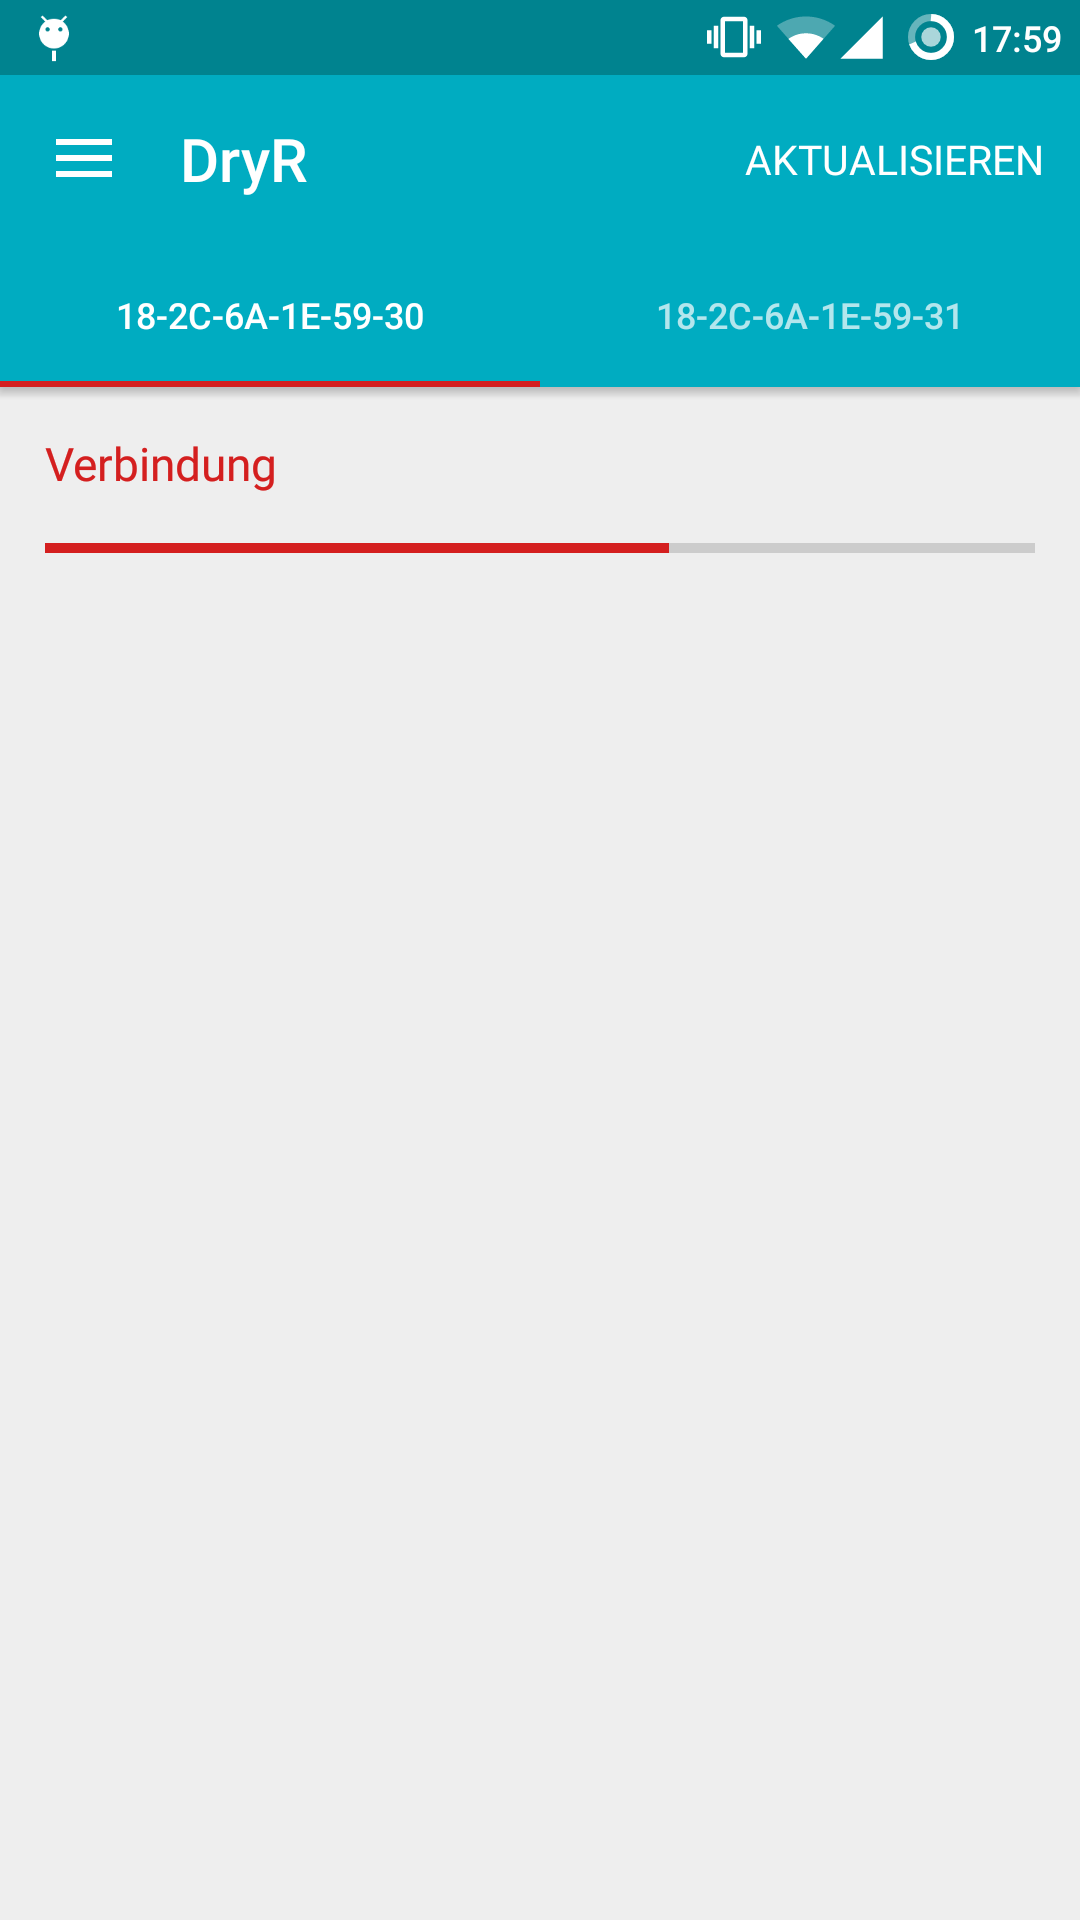
\includegraphics[width=0.7\textwidth]{sensor_status_reception.png}
		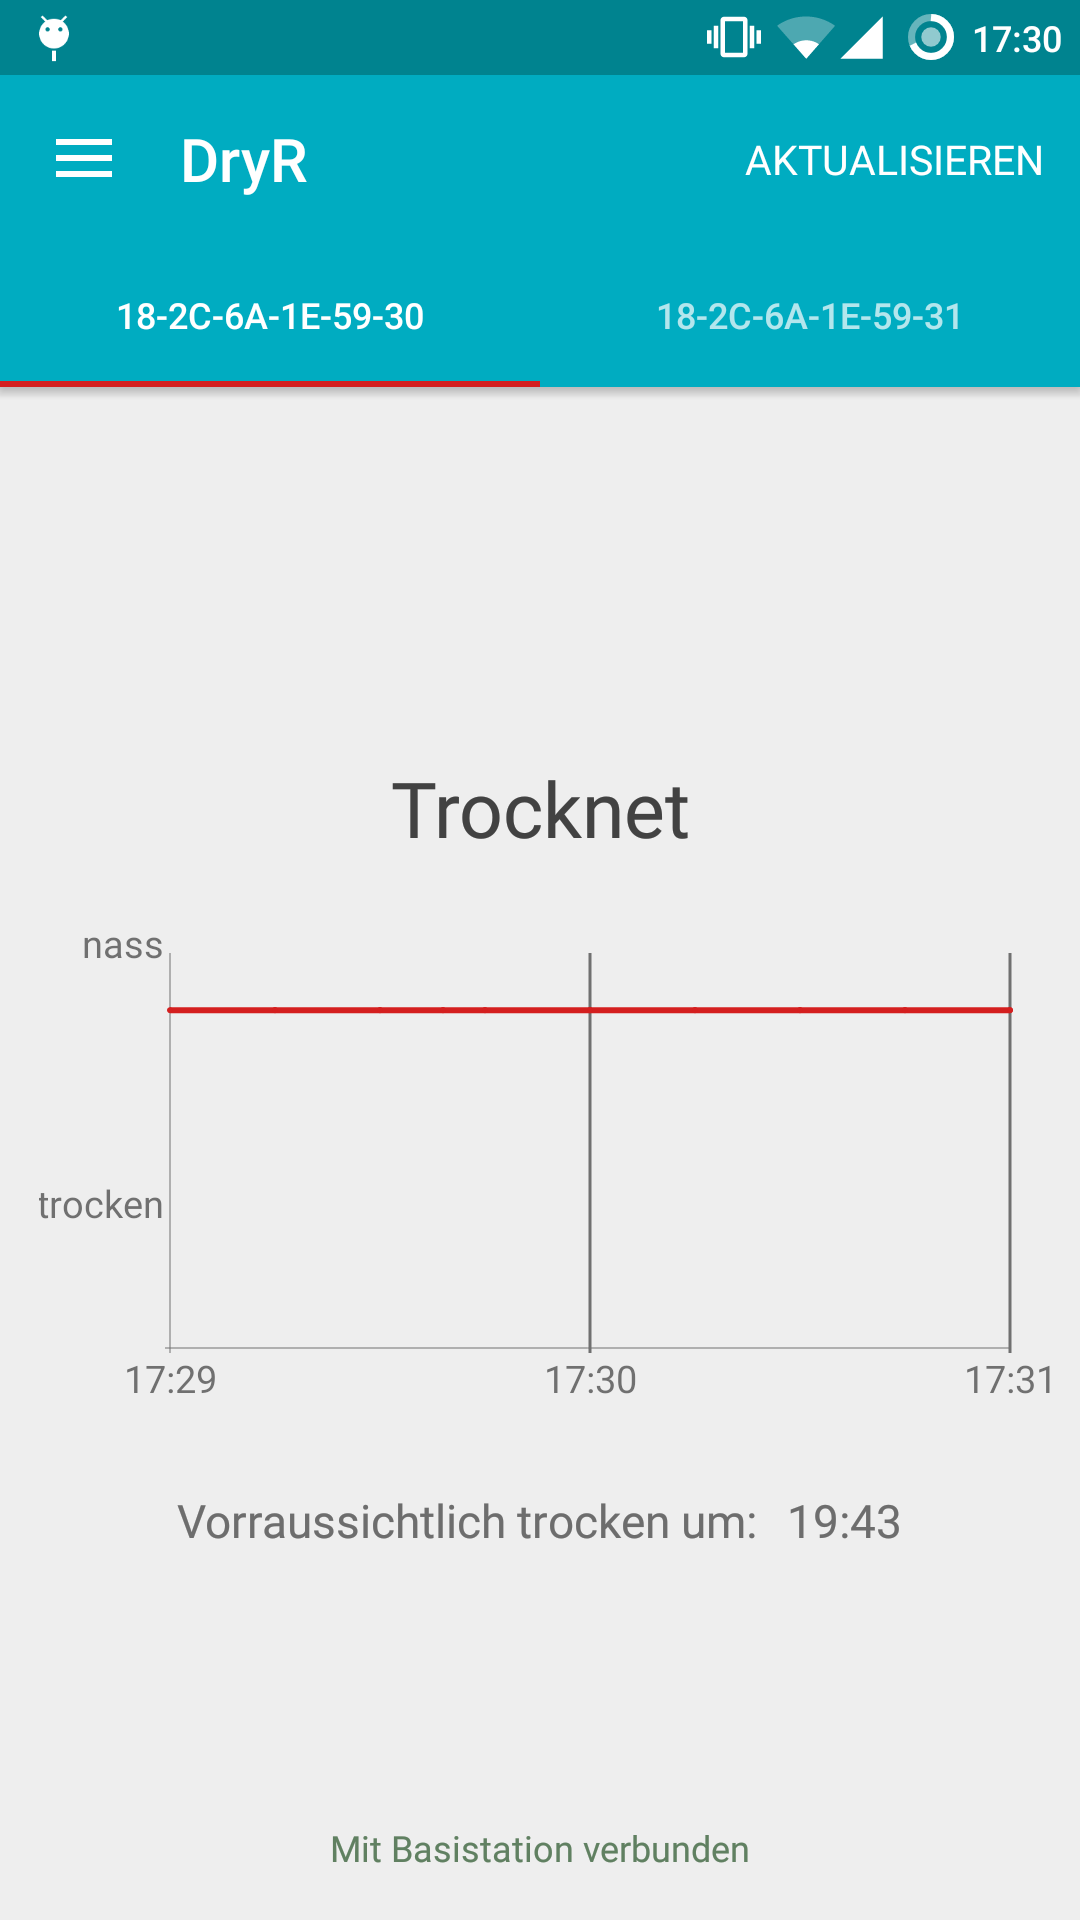
\includegraphics[width=0.7\textwidth]{laundry_status_diagram_forecast.png}
		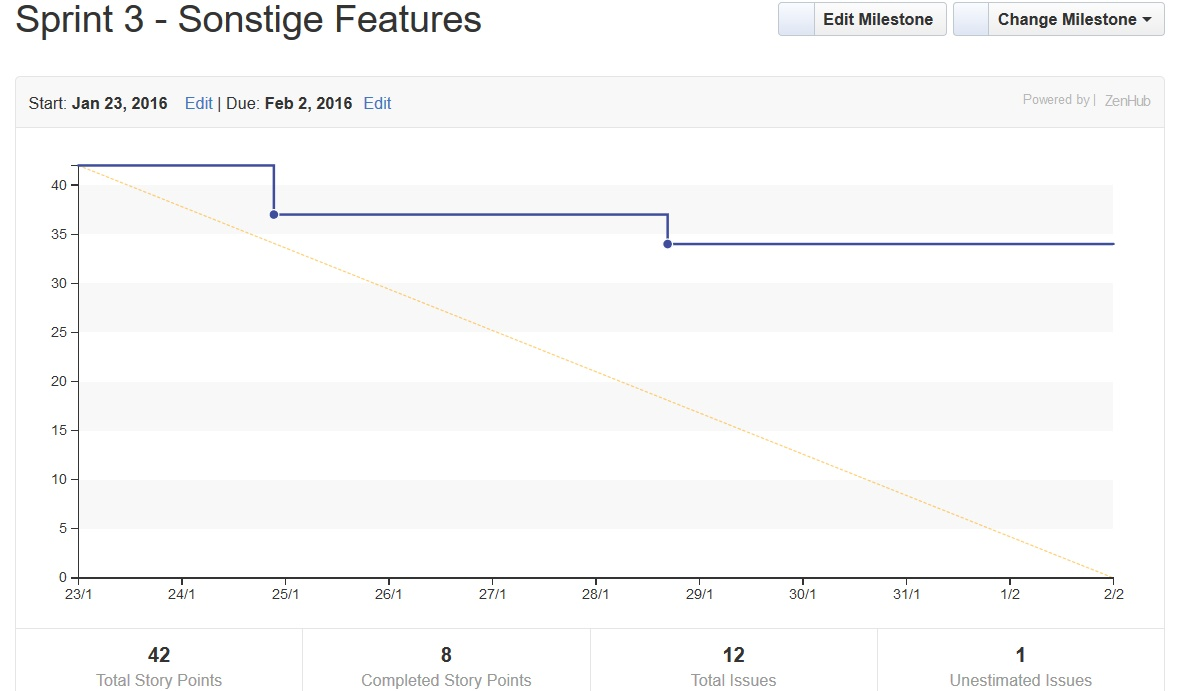
\includegraphics[width=0.7\textwidth]{burndown_sprint3.jpg}
	\item [Features] \hfill \\
		Wir konnten viele Features realisieren. Dazu zählen:
		\begin{description}
			\item [Betrieb mehrer Geräte] Man kann mehrere Klammern mit einer Basisstation auslesen und die App stellt die Klammern da.
			\item [Verbindungsstärke] zeigt an, wie stark die Verbindung zwischen Sensoren und Basisstation ist.
			\item [die Vorhersage] in der man eine geschätzte Uhrzeit gesagt bekommt, zu der die Wäsche trocken ist.
			\item [Benachrichtigung] entweder direkt über Einsicht in die App oder Push.
		\end{description}
		Weggefallen bzw. nicht realisiert wurden:
		\begin{description}
			\item [Benachrichtigung] über Twitter, LED (am Sensor) oder Email. Lässt sich vielleicht noch bei einem Martkreifn Produkt realisieren.
			\item [Regenerkennung] Wir gingen beim Prototypen erstmal nur vom Betrieb in geschlossenen Räumen aus.
			\item [Multi-User] Mehrere Benutzer bekommen Meldungen von einer Basisstation (für Wohngemeinschaften z. B.).
			\item [Ladezustand] Hardware der Sensorplatine war für eine Messung nicht ausgelegt
		\end{description}
\end{description}